\begin{tikzpicture} 
	\node (input0) at (2,6.0) {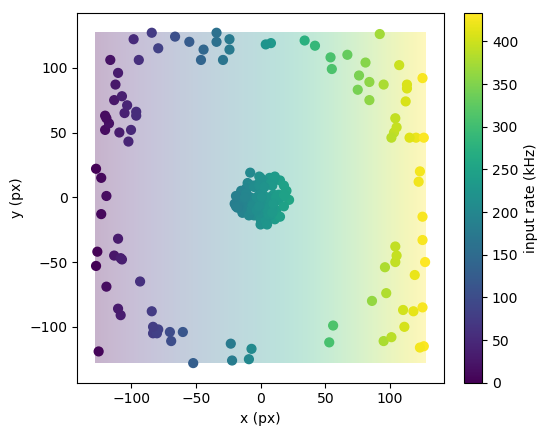
\includegraphics[width=2cm]{learning_process/input_x_map.png}}; 
	\node (input1) at (8,6.0) {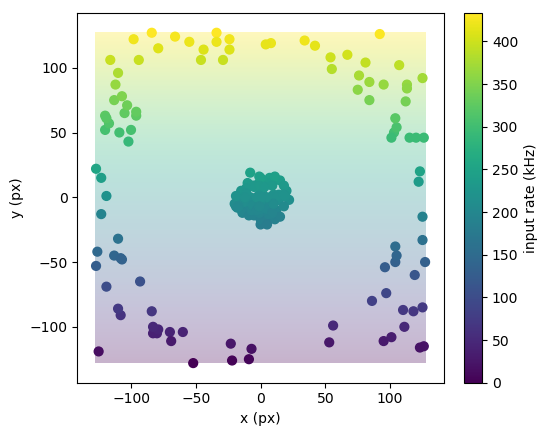
\includegraphics[width=2cm]{learning_process/input_y_map.png}}; 
	\node (hidden0) at (0.0,3.0) {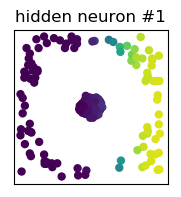
\includegraphics[width=1cm]{learning_process/h_neuron_2500_1.png}}; 
	\node (hidden1) at (1.0,3.0) {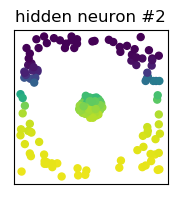
\includegraphics[width=1cm]{learning_process/h_neuron_2500_2.png}}; 
	\node (hidden2) at (2.0,3.0) {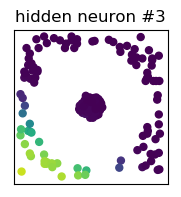
\includegraphics[width=1cm]{learning_process/h_neuron_2500_3.png}}; 
	\node (hidden3) at (3.0,3.0) {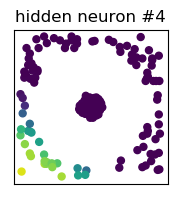
\includegraphics[width=1cm]{learning_process/h_neuron_2500_4.png}}; 
	\node (hidden4) at (4.0,3.0) {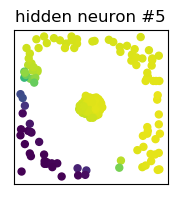
\includegraphics[width=1cm]{learning_process/h_neuron_2500_5.png}}; 
	\node (hidden5) at (5.0,3.0) {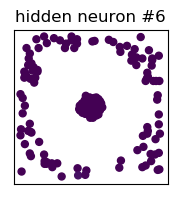
\includegraphics[width=1cm]{learning_process/h_neuron_2500_6.png}}; 
	\node (hidden6) at (6.0,3.0) {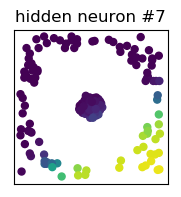
\includegraphics[width=1cm]{learning_process/h_neuron_2500_7.png}}; 
	\node (hidden7) at (7.0,3.0) {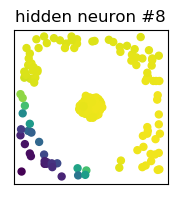
\includegraphics[width=1cm]{learning_process/h_neuron_2500_8.png}}; 
	\node (hidden8) at (8.0,3.0) {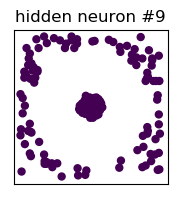
\includegraphics[width=1cm]{learning_process/h_neuron_2500_9.png}}; 
	\node (hidden9) at (9.0,3.0) {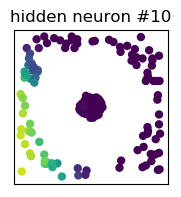
\includegraphics[width=1cm]{learning_process/h_neuron_2500_10.png}}; 
	\node (hidden10) at (10.0,3.0) {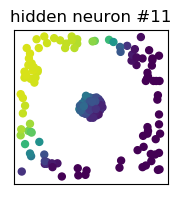
\includegraphics[width=1cm]{learning_process/h_neuron_2500_11.png}}; 
 
	\node (out2500) at (5.5,0.0) {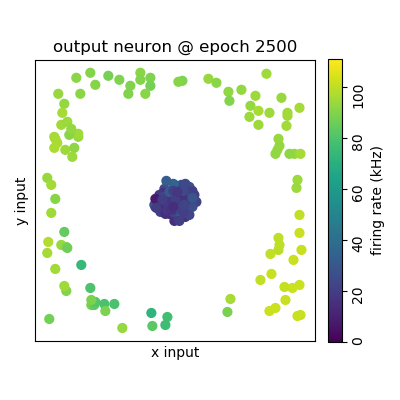
\includegraphics[width=3.6cm]{learning_process/output_neuron_2500.png}}; 
	\draw[-stealth,red!100!white,line width=2.5pt] (input0.south) -- (hidden0.north); 
	\draw[-stealth,red!100!white,line width=0.2pt] (input1.south) -- (hidden0.north); 
	\draw[-stealth,gray!100!white,line width=0.0pt] (input0.south) -- (hidden1.north); 
	\draw[-stealth,blue!100!white,line width=3.1pt] (input1.south) -- (hidden1.north); 
	\draw[-stealth,blue!100!white,line width=1.4pt] (input0.south) -- (hidden2.north); 
	\draw[-stealth,blue!100!white,line width=2.1pt] (input1.south) -- (hidden2.north); 
	\draw[-stealth,blue!100!white,line width=2.4pt] (input0.south) -- (hidden3.north); 
	\draw[-stealth,blue!100!white,line width=2.8pt] (input1.south) -- (hidden3.north); 
	\draw[-stealth,red!100!white,line width=3.0pt] (input0.south) -- (hidden4.north); 
	\draw[-stealth,red!100!white,line width=3.2pt] (input1.south) -- (hidden4.north); 
	\draw[-stealth,gray!100!white,line width=0.0pt] (input0.south) -- (hidden5.north); 
	\draw[-stealth,blue!100!white,line width=1.2pt] (input1.south) -- (hidden5.north); 
	\draw[-stealth,red!100!white,line width=1.8pt] (input0.south) -- (hidden6.north); 
	\draw[-stealth,blue!100!white,line width=2.5pt] (input1.south) -- (hidden6.north); 
	\draw[-stealth,red!100!white,line width=3.1pt] (input0.south) -- (hidden7.north); 
	\draw[-stealth,red!100!white,line width=3.1pt] (input1.south) -- (hidden7.north); 
	\draw[-stealth,red!100!white,line width=0.6pt] (input0.south) -- (hidden8.north); 
	\draw[-stealth,red!100!white,line width=0.3pt] (input1.south) -- (hidden8.north); 
	\draw[-stealth,blue!100!white,line width=3.1pt] (input0.south) -- (hidden9.north); 
	\draw[-stealth,blue!100!white,line width=1.0pt] (input1.south) -- (hidden9.north); 
	\draw[-stealth,blue!100!white,line width=2.5pt] (input0.south) -- (hidden10.north); 
	\draw[-stealth,red!100!white,line width=2.0pt] (input1.south) -- (hidden10.north); 
	\draw[-stealth,line width=2.5pt, color=red ] (hidden0.south) -- (out2500); 
	\draw[-stealth,line width=1.9pt, color=blue ] (hidden1.south) -- (out2500); 
	\draw[-stealth,line width=0.1pt, color=red ] (hidden2.south) -- (out2500); 
	\draw[-stealth,line width=2.1pt, color=red ] (hidden3.south) -- (out2500); 
	\draw[-stealth,line width=1.2pt, color=red ] (hidden4.south) -- (out2500); 
	\draw[-stealth,line width=1.2pt, color=red ] (hidden5.south) -- (out2500); 
	\draw[-stealth,line width=2.6pt, color=red ] (hidden6.south) -- (out2500); 
	\draw[-stealth,line width=0.7pt, color=red ] (hidden7.south) -- (out2500); 
	\draw[-stealth,line width=0.3pt, color=blue ] (hidden8.south) -- (out2500); 
	\draw[-stealth,line width=2.5pt, color=red ] (hidden9.south) -- (out2500); 
	\draw[-stealth,line width=1.7pt, color=red ] (hidden10.south) -- (out2500); 
\end{tikzpicture} 
